% Fra forsiden: CLRS refererer til kursets lærebog, Introduction to Algorithms, 3. udgave.
\section*{Multiple-choice}\label{sec:mc}

Dine svar skal indtastes i ITX-systemets multiple-choice modul.

\multiplechoicestart

\spoergsmaal{MergeSort og rekursion}
Hvis {\sc MergeSort}$(A,p,r)$, implementeret som i CLRS sektion 2.3, 
bliver kaldt på 4 elementer (dvs. $r-p+1 = 4$) laves det første rekursive kald på en liste af 2 elementer, hvorfra det første rekursive kald laves til en liste med 1 element. På det tidspunkt hvor vi når til bunden af rekursionen er der altså 3 kald af {\sc MergeSort} på rekursionsstakken samtidig.
Hvis {\sc MergeSort}$(A,p,r)$ bliver kaldt på 5 elementer bliver der op til 4 kald samtidig på rekursionsstakken.

\medskip

Antag nu at {\sc MergeSort}$(A,p,r)$ bliver kaldt på 42 elementer (dvs. $r-p+1 = 42$).
Hvor stort bliver det største antal samtidige kald til {\sc Merge-Sort}, dvs.~antal kald på rekursionsstakken?
\etsvar
\mulighederstart
\svar 3 samtidige kald.
\svar 4 samtidige kald.
\svar 5 samtidige kald.
\svar 6 samtidige kald.
\svar 7 samtidige kald. \korrekt
\mulighederslut
\forklaring{Største antal elementer på et kald i rekursionsdybde 1,2,3,\dots\ er henholdsvis 42, 21, 11, 6, 3, 2 og 1. Dvs.~der er op til 7 samtidige kald.}


\spoergsmaal{Korteste-veje træ}
Betragt et korteste veje problem (eng.~\emph{single-source shortest-paths problem}) på en orienteret graf $G=(V,E)$ med vægtfunktion $w: E\rightarrow \mathbb{R}$ og startknude $s$.
Hvilke af følgende egenskaber har et korteste-veje træ (eng.~\emph{shortest-paths tree}) $G'=(V',E')$ altid?
\fleresvar
\mulighederstart
\svar Enhver sti i $G'$ er en korteste vej i $G$. \korrekt
\svar Alle korteste veje i $G$ svarer til en sti i $G'$.
\svar $G'$ er et binært træ med $s$ som rod.
\svar $G'$ er et mindste udspændende træ (eng.~\emph{minimum spanning tree}).
\svar Kan beregnes med Dijkstra's algoritme.
\mulighederslut
\forklaring{Der kan være flere korteste veje mellem $s$ og en knude $v$ (med samme vægt), og korteste-vej træet indeholder netop én af disse. 
Korteste-vej træet er ikke nødvendigvis binært, fx kan vi have en graf hvor alle korteste veje fra $s$ består af én kant, dvs. at $s$ har kanter til $|V'|-1$ knuder.
Et mindste udspændende træ (MST) minimerer summen af kantvægte og indeholder ikke nødvendigvis de korteste veje fra en bestemt knude $s$; betragt fx en uorienteret graf med tre knuder og kanter af vægt 2, 2 og 3 hvor et MST vil indeholde de to kanter af vægt 2, men hvor kanten af længde 3 udgør den korteste vej mellem to af knuderne.
Dijkstra's algoritme er kun garanteret korrekt når der ikke er negative vægte, så hvis dette ikke er tilfældet kan output være forkert. (Man kan i stedet bruge en anden algoritme, fx Bellman-Ford.)
}


\spoergsmaal{Korteste veje}
Betragt korteste veje problemet (eng.~\emph{single-source shortest-paths problem}) med startknude {\bf a} på følgende graf:\nylinie
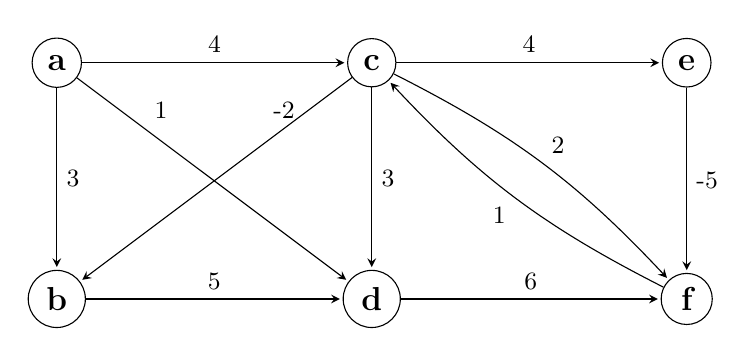
\begin{tikzpicture}[->,>=stealth,shorten >=1pt,auto,
    main node/.style={circle,draw,font=\large\bfseries}]
\node[main node] (a) at (2,1.5) {a};
\node[main node] (b) at (2,-1.5) {b};
\node[main node] (c) at (6,1.5) {c};
\node[main node] (d) at (6,-1.5) {d};
\node[main node] (e) at (10,1.5) {e};
\node[main node] (f) at (10,-1.5) {f};

\path[every node/.style={font=\small}]
(a) edge node {3} (b)
edge node {4} (c)
edge node[pos=0.25] {1} (d)
(b) edge node {5} (d)
(c) edge node {3} (d)
edge [bend left=10] node {2} (f)
edge node {4} (e)
edge node[pos=0.25, above] {-2} (b)
(d) edge node {6} (f)
(e) edge node {-5} (f)
(f) edge [bend left=10] node {1} (c);
\end{tikzpicture}\\
Hvilke kanter er med i korteste-vej træet?
\fleresvar
\mulighederstart
\svar (a,b) 
\svar (a,c) \korrekt
\svar (a,d) \korrekt
\svar (b,d)
\svar (c,b) \korrekt
\svar (c,d)
\svar (c,e) \korrekt
\svar (c,f)
\svar (d,f)
\svar (e,f) \korrekt
\svar (f,c)
\mulighederslut
\forklaring{Da der er negative vægte kan kanterne i træet findes ved at køre Bellman-Ford algoritmen, der giver det angivne output (som i dette tilfælde er unikt).}



\spoergsmaal{Prim's algoritme}
Betragt følgende vægtede, uorienterede graf:
\begin{center}
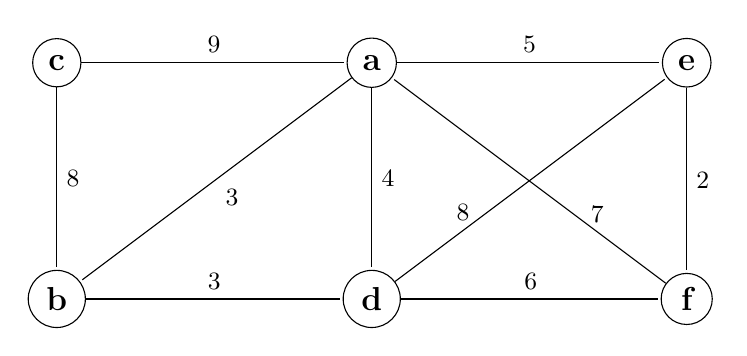
\begin{tikzpicture}[-,>=stealth,shorten >=1pt,auto,
    main node/.style={circle,draw,font=\large\bfseries}]
\node[main node] (a) at (6,1.5) {a};
\node[main node] (b) at (2,-1.5) {b};
\node[main node] (c) at (2,1.5) {c};
\node[main node] (d) at (6,-1.5) {d};
\node[main node] (e) at (10,1.5) {e};
\node[main node] (f) at (10,-1.5) {f};

\path[every node/.style={font=\small}]
(a) edge node {3} (b)
edge node {5} (e)
edge node {4} (d)
(b) edge node {3} (d)
(c) edge node {9} (a)
edge node {8} (b)
(d) edge node {6} (f)
edge node [pos=0.25, above]{8} (e)
(e) edge node {2} (f)
(f) edge node [pos=0.25, above]{7} (a) ;
\end{tikzpicture}
\end{center}
Hvis Prim's algoritme køres på denne graf med start i knude {\bf a}, i hvilken rækkefølge bliver knuderne inkluderet i det mindste udspændende træ? (Med andre ord, i hvilken rækkefølge bliver de taget ud af prioritetskøen?)
\etsvar
\mulighederstart
\svar a, b, d, e, f, c \korrekt
\svar a, b, e, d, f, c % Dijkstra
\svar a, b, d, c, f, e % Sorteret efter vægt
\svar a, b, e, f, d, c % Grådig
\mulighederslut
\forklaring{Håndkørsel af Prim's algoritme og giver den angivne rækkefølge. Bemærk at rækkefølgen \emph{ikke} er den samme som for Dijkstra's algoritme til at finde korteste veje.}



\spoergsmaal{Mindste udspændende træ} 
Betragt mindste udspændende træ (eng.~\emph{minimum spanning tree}) problemet på følgende vægtede, uorienterede graf:\nylinie
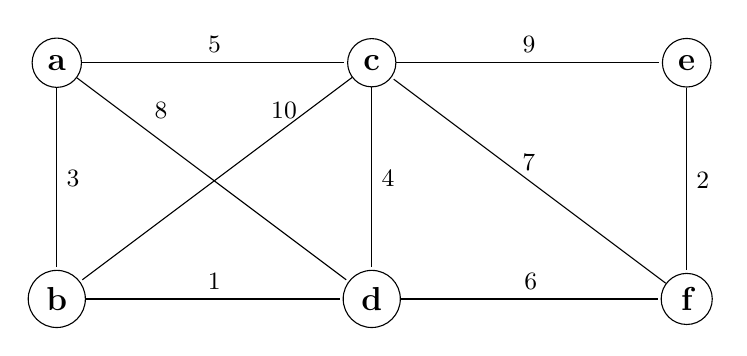
\begin{tikzpicture}[-,>=stealth,shorten >=1pt,auto,
    main node/.style={circle,draw,font=\large\bfseries}]
\node[main node] (a) at (2,1.5) {a};
\node[main node] (b) at (2,-1.5) {b};
\node[main node] (c) at (6,1.5) {c};
\node[main node] (d) at (6,-1.5) {d};
\node[main node] (e) at (10,1.5) {e};
\node[main node] (f) at (10,-1.5) {f};

\path[every node/.style={font=\small}]
(a) edge node {3} (b)
edge node {5} (c)
edge node[pos=0.25] {8} (d)
(b) edge node {1} (d)
(c) edge node {4} (d)
edge node {9} (e)
edge node[pos=0.25, above] {10} (b)
(d) edge node {6} (f)
(e) edge node {2} (f)
(f) edge node[above] {7} (c);
\end{tikzpicture}\\
Hvilke kanter er med i et mindste udspændende træ?
\fleresvar
\mulighederstart
\svar \{a,b\} \korrekt
\svar \{a,c\} 
\svar \{a,d\} 
\svar \{b,d\} \korrekt
\svar \{c,b\} 
\svar \{c,d\} \korrekt
\svar \{c,e\} 
\svar \{c,f\}
\svar \{d,f\} \korrekt
\svar \{e,f\} \korrekt
\mulighederslut
\forklaring{Mindste udspændende træ kan findes ved at køre fx Kruskal's eller Prim's algoritme og giver det angivne output (som i dette tilfælde er unikt).}


\spoergsmaal{Snit og sikre kanter} 
Betragt følgende uorienterede, vægtede graf med knudemængde $V=\{a,b,c,d,e,f\}$:\\
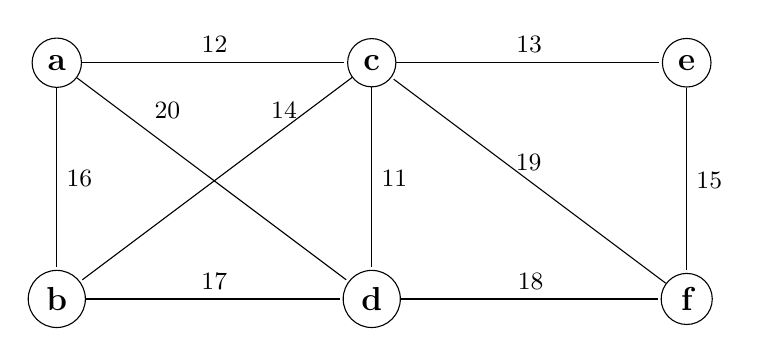
\begin{tikzpicture}[-,>=stealth,shorten >=1pt,auto,
    main node/.style={circle,draw,font=\large\bfseries}]
\node[main node] (a) at (2,1.5) {a};
\node[main node] (b) at (2,-1.5) {b};
\node[main node] (c) at (6,1.5) {c};
\node[main node] (d) at (6,-1.5) {d};
\node[main node] (e) at (10,1.5) {e};
\node[main node] (f) at (10,-1.5) {f};

\path[every node/.style={font=\small}]
(a) edge node {16} (b)
edge node {12} (c)
edge node[pos=0.25] {20} (d)
(b) edge node {17} (d)
(c) edge node {11} (d)
edge node {13} (e)
edge node[pos=0.25, above] {14} (b)
(d) edge node {18} (f)
(e) edge node {15} (f)
(f) edge node[above] {19} (c);
\end{tikzpicture}\\
Betragt kantmængden $A= \{\{a,c\},\{c,d\}\}$, som er en delmængde af et minimalt udspændende træ (eng.~\emph{minimum spanning tree}).
Vi er interesserede i snit (eng.~\emph{cuts}), sikre kanter (eng.~\emph{safe edges}) for $A$, og snit der respekterer (eng.~\emph{respects}) en kantmængde $A$. Hvilke af følgende udsagn er sande?
\fleresvar
\mulighederstart
\svar Lad $S_1=\{a,b,c,d\}$. Snittet $(S_1,V - S_1)$ respekterer kantmængden $A$. \korrekt
\svar Lad $S_2=\{a,c,e\}$. Snittet $(S_2,V - S_2)$ respekterer kantmængden $A$.
\svar Lad $S_3=\{b,e,f\}$. Snittet $(S_3,V - S_3)$ respekterer kantmængden $A$. \korrekt
\svar $\{d,f\}$ er en sikker kant for $A$.
\svar $\{c,e\}$ er en sikker kant for $A$. \korrekt
\svar $\{a,d\}$ er en sikker kant for $A$.
\mulighederslut
\forklaring{ Kanten $\{c,d\}$ krydser snittet $(S_2,V - S_2)$, så det respekterer ikke $A$. 
Snittene med $S_1$ og $S_3$ har ikke nogen kant i $A$, der krydser, så de respekterer $A$.
Kanten $\{d,f\}$ har ikke mindst vægt i snittet $(\{a,c,d\},\{b,e,f\})$, så den er ikke sikker.
Kanten $\{c,e\}$ har mindst vægt i snittet $(\{a,c,d\},\{b,e,f\})$, så den er sikker.
Kanten $\{a,d\}$ krydser ikke snittet $(\{a,c,d\},\{b,e,f\})$, så den er ikke sikker.
}


\spoergsmaal{Amortiseret analyse}
I denne opgave betragter vi potentialfunktionen der bruges til at analysere en binær tæller i CLRS sektion 17.3.
Lad $\Phi(D_i)$ betegne potentialfunktionens værdi efter $i$ {\sc Increment} operationer.
Hvilke egenskaber har $\Phi(D_i)$?
(Læg mærke til at udsagnene ikke er uafhængige --- hvis der gælder $f(i) = \Omega(i)$ så gælder også $f(i) = \Omega(\lg i)$, osv.)
\fleresvar
\mulighederstart
%\svar $\Phi(D_i) = \Omega(1)$. \korrekt Udeladt da potentialet bliver 0 når i=2^k
\svar $\Phi(D_i) = \Omega(\lg i)$.
\svar $\Phi(D_i) = \Omega(i)$.
\svar $\Phi(D_i) = O(1)$.
\svar $\Phi(D_i) = O(\lg i)$. \korrekt
\svar $\Phi(D_i) = O(i)$. \korrekt
\mulighederslut
\forklaring{ $\Phi(D_i)$ er lig med antal 1er i den binære repræsentation af tallet $i$ (som er mindst 1 for $i>0$). Hvis $i$ er en potens af 2 er $\Phi(D_i) = 1$, så vi kan ikke begrænse funktionen nedefra med en voksende funktion af $i$. Hvis $i+1$ en potens af 2 er $\Phi(D_i) = \lg(i+1)$, så både $O(\lg i)$ og $O(i)$ er gyldige øvre grænser.
}



\spoergsmaal{Køretid}
Betragt følgende kode i pseudo-kode notationen fra CLRS:
\begin{codebox}
 \Procname{$\proc{Loops}(n)$}
 \li $r = 0$
 \li \For $i = 1$ \To $n/2$
 \li \Do \For $j = n/2-i$ \To $n$
 \li \Do $r = r + j$ \End \End \End
 \li \Return r
\end{codebox}
Vi antager at $n/2$ er et heltal således at den yderste {\bf for}-løkke har $n/2$ iterationer.
Hvilke af følgende er gyldige udsagn om køretiden $T(n)$ af {\sc Loops}$(n)$?
(Læg mærke til at udsagnene ikke er uafhængige --- hvis der gælder $f(n) = O(n)$ så gælder også $f(n) = O(n \lg n)$, osv.)
\fleresvar
\mulighederstart
\svar $T(n) = O(n)$.
\svar $T(n) = O(n \lg n)$.
\svar $T(n) = O(n^2)$. \korrekt
\svar $T(n) = \Omega(n)$. \korrekt
\svar $T(n) = \Omega(n \lg n)$. \korrekt
\svar $T(n) = \Omega(n^2)$. \korrekt
\mulighederslut

\forklaring{ Der er $n/2$ iterationer af den ydre løkke, der hver tager $O(n)$ tid fordi den indre løkke laver mellem $n/2$ og $n$ iterationer. Dvs.~køretiden er $\Theta(n^2)$. Derfor er de to første store-O grænser for lave, mens de øvrige grænser gælder.}



\spoergsmaal{Rekursionsligninger}
Hvilke af disse rekursionsligninger har løsningen
$T(n) = \Theta(n \lg n)$? Antag at $T(n)=1$ for $n\leq 1$.
\fleresvar
\mulighederstart
\svar $T(n) = 2 T(\lfloor n/2\rfloor ) + n^2$.
\svar $T(n) = 2 T(\lfloor n/2\rfloor ) + 3n$. \korrekt
\svar $T(n) = 2 T(\lfloor n/3\rfloor ) + 2n$.
\svar $T(n) = 3 T(\lfloor n/2\rfloor ) + n \lg n$.
\svar $T(n) = 3 T(\lfloor n/3\rfloor ) + n$. \korrekt
\svar $T(n) = T(n-1) + \lg n$. \korrekt % Kan ikke løses med master theorem i CLRS
\mulighederslut
\forklaring{ De fem første rekursionsligninger kan løses ved hjælp af master theorem, hvor nummer 2 og 5 falder i tilfælde 2 og giver $T(n) = \Theta(n \lg n)$.
Den sidste ligning kan løses med substitutionsmetoden, hvor der er $n$ led af størrelse højst $\lg n$, og hvor halvdelen har størrelse mindst $\lg(n/2) = \lg(n) - 1$.
}



\spoergsmaal{Del og hersk}
Antag at du har en rekursiv algoritme $A$, og lad $n$ betegne størrelsen på algoritmens input~$X$.
Hvis $n=1$ beregnes resultatet $A(X)$ i konstant tid.
For $n>1$ bruger algoritmen først $O(n \lg n)$ tid på at beregne fire inputs $X_1, X_2, X_3, X_4$, hver af størrelse $\lfloor n/2\rfloor$, og $A(X_1), A(X_2), A(X_3), A(X_4)$ beregnes rekursivt.
Endelig kombineres de rekursive svar til et output $A(X)$ i tid $O(n^2)$.

\medskip 

Hvilken af disse rekursionsligninger beskriver køretiden $T(n)$ af $A$ på input $X$?
\etsvar
\mulighederstart
\svar $T(n) = 4 T(\lfloor n/2\rfloor ) + O(n \lg n)$.
\svar $T(n) = 2 T(\lfloor n/4\rfloor ) + O(n \lg n)$.
\svar $T(n) = 4 T(\lfloor n/2\rfloor ) + O(n^2)$. \korrekt
\svar $T(n) = 2 T(\lfloor n/4\rfloor ) + O(n^2)$.
\mulighederslut
\forklaring{ De fire rekursive delproblemer af størrelse $\lfloor n/2\rfloor$ tager total tid $4 T(\lfloor n/2\rfloor )$. Derudover bruges der totalt tid $O(n^2)$ på at beregne $A(X)$.
}



\spoergsmaal{Fibonacci hobe}
Betragt en Fibonacci hob $H$ (eng.~\emph{Fibonacci heap}), som beskrevet i CLRS kapitel 19, hvorpå der udføres $n_1$ {\sc Insert} operationer, $n_2$ {\sc Extract-Min} operationer, og $n_3$ {\sc Decrease-Key} operationer.
Det totale antal operationer er $n=n_1+n_2+n_3$.
Hvilke af følgende udsagn er altid sande?
\fleresvar
\mulighederstart
\svar Den samlede worst case tid for operationerne er $\Omega(n \lg n)$.
\svar Den samlede worst case tid for operationerne er $O(n \lg n)$. \korrekt
\svar Den samlede worst case tid for operationerne er $O(n_1 + n_3 + n_2 \lg n)$. \korrekt
\svar $H$ har $n_1 - n_2 - n_3$ knuder.
\svar $H$ har $m(H) = n_1 - n_2$ markerede knuder.
\mulighederslut
\forklaring{ Den amortiserede analyse giver en øvre grænse på $O(n_1 + n_3 + n_2 \lg n)$ for operationerne. Da $n=n_1+n_2+n_3$ er det specielt $O(n \lg n)$. Hvis $n_1 + n_3 > n_2\lg n$ bliver tiden $O(n)$, så tiden er ikke nødvendigvis $\Omega(n \lg n)$. Antal knuder i $H$ er antal indsættelser minus antal sletninger, dvs. $n_1 - n_2$ som er forskellig fra $n_1 - n_2 - n_3$ hvis $n_3 >0$.
Antal markerede knuder kan ikke udtrykkes ved hjælp af $n_1$ og $n_2$ --- for eksempel ændrer {\sc Insert} ikke antallet af markerede knuder.
}



\spoergsmaal{Binære søgetræer}\label{q:red-black}
Betragt et rød-sort binært søgetræ $T$ (eng.~\emph{red-black binary search tree}), som beskrevet i CLRS kapitel 13.
Betragt nedenstående træ, hvor alle blade er udeladt (som på CLRS figur 13.1.c) og to indre knuder er uspecificerede:

\begin{center}
\begin{tikzpicture}[-,>=stealth,level/.style={sibling distance = 5cm/#1,
    level distance = 1cm}] 
  \node [black] {42}
      child{ node [red] {24} 
              child{ node [black] {19} 
                  child{ node [red] {14} }
                  child{ node [white] {}}
              }
              child{ node [gray] {?}
                              child{ node [red] {27}}
                              child{ node [red] {31}}
              }                            
      }
      child{ node [black] {56}
              child{ node [red] {47} 
              }
              child{ node [white] {?}
              }
          }
  ; 
  \end{tikzpicture}  
\end{center}

\medskip

Hvilke knuder er mulige på mindst én af positionerne markeret med ?, hvis træet skal overholde invarianterne for et rød-sort binært søgetræ?
\fleresvar
\mulighederstart
\svar En rød knude med nøglen 28.
\svar En rød knude med nøglen 44.
\svar En rød knude med nøglen 58. \korrekt
\svar En sort knude med nøglen 25.
\svar En sort knude med nøglen 30. \korrekt
\svar En sort knude med nøglen 66.
\mulighederslut
\forklaring{ Knuden til venstre skal være sort (fordi røde knuder har sorte børn) og ligge mellem 27 og 31. Derfor er kun en sort knude med nøglen 30 en mulighed hér. Knuden til højre skal være rød (fordi alle stier fra roden skal have samme antal sorte knuder) og større end 56, så kun en rød knude med nøglen 58 er mulig hér.
}



\spoergsmaal{Binære søgetræer}
Betragt dette rød-sorte binære søgetræ (igen med bladene udeladt):
%
\begin{center}
\begin{tikzpicture}[-,>=stealth,level/.style={sibling distance = 5cm/#1,
    level distance = 1cm}] 
  \node [black] {40}
      child{ node [black] {24} 
              child{ node [red] {19} 
              }
              child{ node [red] {39}
              }                            
      }
      child{ node [red] {56}
              child{ node [black] {47} 
              }
              child{ node [black] {77}
              }
          }
  ; 
  \end{tikzpicture}  
\end{center}

\medskip

Antag at vi bruger indsættelsesalgoritmen {\sc RB-Insert} fra CLRS kapitel 13 til at indsætte nøglen~42. Hvad sker med træet?
\etsvar
\mulighederstart
\svar 42 indsættes som en sort knude under knuden 47.
\svar 42 indsættes som en rød knude under knuden 47. \korrekt
\svar 42 indsættes som ny sort rodknude og 40 bliver barn til knuden 39.
\svar 42 indsættes som ny rød rodknude og 40 bliver barn til knuden 39.
\svar Ingen af ovenstående.
\mulighederslut
\forklaring{ {\sc RB-Insert} finder det rette sted i træet til nøglen 42, som det venstre barn under knude 47. Knuden farves rød og derefter kaldes {\sc RB-Insert-Fixup}, men den terminerer uden at ændre noget fordi forældreknuden 47 er sort.
}


\spoergsmaal{Disjunkte mængder}
Vi betragter trærepræsentationer af disjunkte mængder (eng.~\emph{disjoint sets}), som beskrevet i CLRS sektion 21.3, ved brug af heuristikkerne \emph{union by rank} og \emph{path compression}.
Antag at {\sc Make-Set} er kørt $n$ gange og lad $k$ være en variabel.
Hvilke af følgende udsagn er altid sande?
\fleresvar
\mulighederstart
\svar Tiden for et kald til {\sc Union}$(x,y)$ er $O(\lg n)$. \korrekt
\svar $k$ kald til {\sc Find-Set}$(42)$ lige efter hinanden tager tid $O(k + \lg n)$. \korrekt
\svar Kaldene {\sc Make-Set}$(x_1)$,\dots,{\sc Make-Set}$(x_k)$ tager total tid $O(k)$. \korrekt
\svar En {\sc Link}$(x,y)$ operation øger den maksimale værdi af \emph{rank} i træerne for $x$ og $y$ med~1.
\svar I værste fald tager en {\sc Find-Set} operation $\Omega(n)$ tid.
\svar {\sc Union}$(x,x)$ tager konstant tid.
\mulighederslut
\forklaring{ Dybden af trærepræsentationen er $O(\lg n)$, så det gælder også tiden for {\sc Find-Set} og dermed {\sc Union}.
Kalder vi {\sc Find-Set}(42) igen efter at den lige er blevet kaldt vil operationen tage konstant tid, dvs.~tiden for $k$ kald bliver $O(k + \lg n)$. En {\sc Link} operation giver kun en større \emph{rank} hvis røddernes rank er identisk.
Med den givne implementation af {\sc Union}$(x,x)$ laves der to kald til {\sc Find-Set}, der ikke nødvendigvis tager konstant tid.
}


\spoergsmaal{Invarianter}
Betragt følgende funktion, i pseudo-kode notationen fra CLRS, hvor input $A$ er en tabel af heltal og $n$ er længden af $A$.
\begin{codebox}
  \Procname{$\proc{Second-Smallest}(A, n)$}
  \li $m = A[1]$
  \li $r = \infty$
  \li \For $i = 2$ \To $n$
  \li \Do \If $A[i] < m$  
  \li         \Then $r = m$
  \li         $m = A[i]$ 
  \li       \ElseIf $A[i] < r$
  \li     \Then $r = A[i]$  \End \End \End
  \li \Return $r$
\end{codebox}

\noindent
Hvilke udsagn gyldige løkke-invarianter ved starten af hver iteration i {\bf for}-løkken?
\fleresvar
\mulighederstart
\svar $m = \min(A[1],\dots,A[i-1])$. \korrekt
\svar $m = \min(A[1],\dots,A[n])$.
\svar $r \geq m$. \korrekt
\svar $m \geq 0$.
\svar Mindst 1 element i $A[1],\dots,A[i-1]$ er mindre end eller lig med $r$. \korrekt
\svar Højst 2 elementer i $A[1],\dots,A[i-1]$ er mindre end eller lig med $r$.
\mulighederslut

\forklaring{ Udsagn 1, 3 og 5 gælder for $i=2$ pga.~initialiseringen af $m$ og $r$, og kan ses at gælde efter hver iteration ved induktion. Udsagn 2 gælder ikke hvis minimum i $A$ ikke er lig med $A[1]$. Udsagn 4 gælder ikke hvis $A[1]<0$. Udsagn 6 gælder ikke hvis der er 3 værdier i $A$, der har den samme, mindste værdi. }



\spoergsmaal{Valg af datastruktur}
Antag at vi gerne vil skabe en datastruktur {\sc Ventetid}, der indeholder en mængde af $n$ afgangstidspunkter (ugedag og klokkeslet, fx for en bus).
For enkelheds skyld skal der blot holdes styr på én rute og ét stoppested, så den eneste information er afgangstidspunkter.
Datastrukturen skal understøtte to operationer: {\sc Insert}$(x)$, der indsætter et nyt afgangstidspunkt, og {\sc HvorLænge}$(x)$ der returnerer antal minutter fra tidspunkt $x$ til den næste afgang.

\medskip

Hvad er det mest passende valg af datastruktur til løsning af dette problem blandt nedenstående, og hvilken worst-case (amortiseret) køretid for {\sc HvorLænge}$(x)$ bliver resultatet af dette valg?
Udtryk svaret som funktion af $n$.
\etsvar
\mulighederstart
\svar Disjunkte mængder (eng.~\emph{disjoint sets}), tid $O(1)$.
\svar Disjunkte mængder (eng.~\emph{disjoint sets}), tid $O(\lg n)$.
\svar Fibonacci hob (eng.~\emph{Fibonacci heap}), tid $O(\lg n)$.
\svar Fibonacci hob (eng.~\emph{Fibonacci heap}), tid $O(1)$.
\svar Rød-sort binært søgetræ (eng.~\emph{red-black binary search tree}), tid $O(\lg n)$. \korrekt
\svar Rød-sort binært søgetræ (eng.~\emph{red-black binary search tree}), tid $O(1)$.
\mulighederslut

\forklaring{ Hvis vi indsætter afgangstiderne i et rød-sort søgetræ så kan {\sc HvorLænge}$(x)$ implementeres som et kald til {\sc Successor}$(x)$. Hvis der ikke findes nogen efterfølger til $x$ (fordi der ikke er nogen senere afgang i samme uge), returneres minimum, dvs.~den første afgang i næste uge. I begge tilfælde tager det tid $O(\log n)$. }



\spoergsmaal{Korrekthedsargumenter}\label{sec:maxproduct}
Betragt følgende problem, kaldet {\tt MaxProduct}: 
\newcommand{\maxproductproblem}{
Givet en liste af tal $x_1,\dots,x_n \in {\bf R}$ (kan være både positive og negative),
find en delmængde $I^*\subseteq \{1,\dots,n\}$ hvor produktet $\prod_{i\in I^*} x_i$ er så stort som muligt, dvs. for alle mængder $I\subseteq \{1,\dots,n\}$ skal gælde at $\prod_{i\in I} x_i \leq \prod_{i\in I^*} x_i$.

\medskip

{\bf Eksempel.} På input $x_1=-4,\, x_2=-0.5,\, x_3=0.5,\, x_4=0.5,\, x_5=1.5,\, x_6=6$ kan vi vælge $I=\{5,6\}$ og få et produkt på $1.5\cdot 6 = 9$, men et bedre valg er $I=\{1,2,5,6\}$ som giver produktet $(-4) \cdot (-0.5) \cdot 1.5\cdot 6 = 18$. Den tomme mængde $I=\emptyset$ giver per definition $\prod_{i\in \emptyset} x_i = 1$.
}

\maxproductproblem

\medskip

\noindent
Hvad gælder altid for en optimal løsning $I^*$?
\fleresvar
\mulighederstart
\svar $I^*$ indeholder \emph{ikke} noget indeks $i$ hvor $x_i$ er mellem 0 og 1 ($x_i\in (0,1))$. \korrekt
\svar $I^*$ indeholder \emph{alle} indekser $i$ hvor $x_i < 0$.
\svar $I^*$ indeholder \emph{alle} indekser $i$ hvor $x_i > 1$. \korrekt
\svar $I^*$ indeholder \emph{alle} indekser $i$ hvor $|x_i| > 1$ (i.e., absolutværdien af $x_i$ er større end 1).
\mulighederslut
\forklaring{
Den optimale løsning har altid produkt mindst $1$ fordi vi kan vælge $I=\emptyset$.
Hvis $I^*$ indeholdt $i$ hvor $x_i \in (0,1)$ så kunne man opnå et større produkt ved at vælge $I=I^*\backslash \{i\}$, hvilket er en modstrid.
Hvis antallet af negative indeks er ulige kan vi ikke have dem alle med i en optimal løsning, da produktet så ville blive negativt.
Hvis vi udelader et indeks med $x_i > 1$, så $i\not\in I^*$ kan vi opnå et større produkt ved at vælge $I=I^* \cup \{i\}$, hvilket er en modstrid.
Hvis antallet af indeks i med $x_i < -1$ er ulige kan vi ikke have dem alle med i en optimal løsning, da produktet så ville blive negativt.
}



\spoergsmaal{Dynamisk programmering}
En \emph{stigende delsekvens} af en tabel $A$, der indeholder heltal $A[1],\dots,A[n]$, er en delmængde af indekser $1\leq i_1 < i_2 < \dots < i_k \leq n$ således at $A[i_1] < A[i_2] < \dots < A[i_k]$.
Længden af delsekvensen er antal indekser, $k$.
En \emph{ikke-aftagende delsekvens} defineres på samme måde bortset fra at kravet er $A[i_1] \leq A[i_2] \leq \dots \leq A[i_k]$.
Betragt følgende funktion, i pseudo-kode notationen fra CLRS, hvor input $A$ er en tabel af heltal.
\begin{codebox}
  \Procname{$\proc{MaximumMystery}(A,n)$}
  \li let $r[1\dots n]$ be a new array
  \li $r[1] = 1$
  \li \For $j = 2$ \To $n$
  \li \Do $q \gets 1$
  \li \For $i=1$ \To $j-1$
  \li \Do \If {\bf not} $A[j] < A[i]$
  \li \Then $q = \max(q, r[i] + 1)$ \End\End
  \li $r[j]=q$ \End
  \li \Return $\max(r[1],\dots,r[n])$
\end{codebox}

\noindent
Hvad beregner proceduren {\sc MaximumMystery}?
\etsvar
\mulighederstart
\svar Indekserne i en længste stigende delsekvens.
\svar Indekserne i en længste ikke-aftagende delsekvens.
\svar Længden af en længste stigende delsekvens.
\svar Længden af en længste ikke-aftagende delsekvens. \korrekt
\mulighederslut

\forklaring{ Invarianten for den ydre løkke er at for $\ell = 1,\dots,j-1$ er $r[\ell]$ længden af en længste ikke-aftagende delsekvens, der slutter i indekset $\ell$. Den indre løkke beregner $r[j]$ ved rekursionsformlen $r[j] = 1 + \underset{i<j,\, A[i]\leq A[j]}{\max} r[i]$, hvor maximum af den tomme mængde defineres som 0. Hvis $A[j]$ er mindre end alle tidligere værdier i $A$ beholdes initialiseringsværdien $q = 1$. En længste ikke-aftagende delsekvens slutter i et eller andet indeks, så dens længde er $\max(r[1],\dots,r[n])$.}




\multiplechoiceslut

\newpage


\section*{Skriftlige opgaver}\label{sec:written}

{\bf Skriftlige opgaver} afleveres som et Word dokument i ITX systemet.
Der er mulighed for at tegne og skrive på tablet, og indsætte i dokumentet.
\begin{itemize}
    \item Brug \emph{én side til hvert delspørgsmål, i samme rækkefølge som i opgavesættet.} 
    \item Delspørgsmålets nummer/bogstav (fx 19 eller 20.a) skal fremgå.
\end{itemize}



\section{Længste fælles delsekvens (4\%)}

Vi betragter algoritmen til længste fælles delsekvens (eng.~\emph{longest common subsequence}) i CLRS sektion 15.4.

\punkt{a)}{
Tegn tabellen $c$ som algoritmen udfylder på følgende input:
\begin{center}
$x=\langle N,A,A,N\rangle$ og $y=\langle A,N,N,A\rangle$.
\end{center}
\medskip
\noindent
Tilføj pile ($\uparrow$, $\nwarrow$, $\leftarrow$), der forklarer tallene i tabellen, som i CLRS Figur 15.8 og angiv den længste fælles delsekvens.
}

\forklaring{For overskuelighedens skyld inkluderer vi de to strenge i kanten af tabellen $c$, ligesom i CLRS Figur 15.8.\medskip
\begin{center}
\begin{tabular}{c||c|c|c|c|c||}
    & & A & N & N & A\\
    \hline
    \hline
     & 0 & 0 & 0 & 0 & 0\\
     \hline
    N & 0 & $\uparrow$0 & $\nwarrow$1 & $\nwarrow$1 & $\leftarrow$1 \\
    \hline
    A & 0 & $\nwarrow$1 & $\uparrow$1 & $\uparrow$1 & $\nwarrow$2 \\
    \hline
    A & 0 & $\nwarrow$1 & $\uparrow$1 & $\uparrow$1 & $\nwarrow$2 \\
    \hline
    N & 0 & $\uparrow$1 & $\nwarrow$2 & $\nwarrow$2 & $\uparrow$2 \\
    \hline
    \hline
\end{tabular}
\end{center}
(I nogle tilfælde er der et valg mellem $\uparrow$ og $\leftarrow$, det lægger vi ikke vægt på når der gives point.) Længste fælles delsekvens er NA.
}


\section{Dynamisk programmering (10\%)}

Vi betragter følgende variant af længste fælles delsekvens (eng. \emph{longest common subsequence}) problemet fra CLRS sektion 15.4.
Input er to vektorer $x=\langle x_1,\dots,x_m\rangle \in \Sigma^m$ og $y=\langle y_1,\dots,y_n\rangle \in \Sigma^n$.
I lighed med længste fælles delsekvens er målet at finde en optimal vektor $z=\langle z_1,\dots,z_k\rangle$, men i stedet for at maksimere længden af $z$ skal \emph{vægten} af tegnene i $z$ maksimeres.
Vi antager at vægtene er ikke-negative.
Vægten er givet ved en datastruktur $w$, således at vægten af $z_i \in\Sigma$, der betegnes med $w[z_i]$, kan findes i konstant tid.
Vægten af $z$ er summen af vægte, $\sum_{i=1}^k w[z_i]$, og målet er et finde en fælles delsekvens med størst mulig vægt.

\medskip

{\bf Eksempel.} Antag at vi har $x=\langle A, H, A, A \rangle$, $y=\langle A, A, R, G, H \rangle$, og $w[A] = 2$, $w[G]=8$, $w[R] = 10$, $w[H] = 5$. Delsekvensen $\langle A, A \rangle$ med vægt $2+2 = 4$ findes i både $x$ og $y$. Delsekvensen $\langle A, H \rangle$ med vægt $2+5 = 7$ findes også i både $x$ og $y$, og er den delsekvens, der har størst vægt.


\punkt{a)}{Skriv en rekursionsligning for den optimale vægt af en fælles delsekvens af $x$ og $y$.}

\forklaring{ I forhold til det almindelige længste fælles delsekvens problem skal vi ændre omkostningen i det tilfælde hvor to karakterer matcher så det afspejler vægten:
%
\begin{equation*}
    c[i,j] = \begin{cases}
    0 &\text{hvis } i=0 \text{ eller } j=0\\
    c[i-1,j-1] + w[\alpha] & \text{hvis } i,j>0 \text{ og } x_i = y_j = \alpha\\
    \max(c[i-1,j], c[i,j-1]) & \text{hvis } i,j>0 \text{ og } x_i \ne y_j\\
    \end{cases}
\end{equation*}
}

\punkt{b)}{Lav en analyse af køretiden af den algoritme, der bruger rekursionsligningen og dynamisk programmering til at beregne den optimale vægt.
Analysen skal give en øvre grænse på køretiden som funktion af $n$ og $m$ i store-$O$ notation, der er så præcis som mulig.
}

\forklaring{Analysen for længste fælles delsekvens kan genbruges, da rekursionsligningen har samme struktur. Ændringen påvirker kun værdierne og tiden for hvert skridt øges med højst en konstant faktor (da en vægt kan findes i konstant tid). Derfor er køretiden $O(n m)$.}

\punkt{c)}{Beskriv hvordan algoritmen kan modificeres til at håndtere det tilfælde hvor vægte kan være negative uden at påvirke den asymptotiske køretid. Argumentér for køretid og korrekthed af din løsning.}

\forklaring{Tegn med negative vægte vil aldrig være del af en optimal løsning, hvilket kan ses med et modstridsargument: Hvis $z$ indeholder et tegn med negativ vægt, så har delsekvensen der udelader dette element højere vægt.
Tegn med negativ vægt kan derfor fjernes fra input i tid $O(n+m)$, hvorefter det resterende problem er uden negative vægte.
Den samlede tid er $O(n+m+nm)$, hvilket er $O(nm)$ som inden.}





\section{Induktionsbeviser (6\%)}

I denne opgave antager vi at $T$ er en sorteret tabel med $n > 1$ elementer således at for $i<j$ gælder $T[i] \leq T[j]$.
Antag at $1\leq p\leq r\leq n$.
Betragt følgende funktion, i pseudo-kode notationen fra CLRS:
%
\begin{codebox}
  \Procname{$\proc{WhileMystery}(x, T, p, r)$}
  \li $low = p$
  \li $high = \max(p,r+1)$
  \li \While $low < high$
  \li \Do $mid = \lfloor (low+high)/2\rfloor$
  \li \If $x \leq T[mid]$ \Then
  \li $high = mid$
  \li \Else
  \li $low = mid + 1$ \End \End
  \li \Return $high$
\end{codebox}

\punkt{a)}{Lad $high_i$ og $low_i$ betegne værdien af variablene $high$ og $low$ efter $i$ iterationer af {\bf while} løkken.  
Bevis ved induktion at $high_i-low_i \leq n/2^i$. (Du skal bruge antagelsen $1\leq p\leq r\leq n$.) Der lægges vægt på, at argumentationen er klar og koncis.}

\forklaring{ 
Inden den første iteration har vi $high_0 - low_0 = \max(p,r+1) - p \leq n = n/2^0$. 
Det viser basistilfældet $i=0$.
I induktionsskridtet antager vi, at efter $i-1$ iterationer gælder $high_{i-1}-low_{i-1} \leq n/2^{i-1}$.
Efter iteration $i$ er vi i ét at to tilfælde afhængigt af udfaldes af sammenligningen i linje 5:
 $high_i = \lfloor (low_{i-1}+high_{i-1})/2\rfloor$ og $low_i = low_{i-1}$ eller
$low_i = \lfloor (low_{i-1}+high_{i-1})/2\rfloor + 1$ og $high_i = high_{i-1}$.
I det første tilfælde har vi, via induktionshypotesen:
\[ high_i-low_i = \lfloor (low_{i-1}+high_{i-1})/2\rfloor - low_{i-1} \leq (high_{i-1} - low_{i-1})/2 \leq (n/2^{i-1})/2 = n/2^{i} \enspace .\]
I det andet tilfælde har vi:
\[ high_i-low_i = high_{i-1} - (\lfloor (low_{i-1}+high_{i-1})/2\rfloor + 1) \leq (high_{i-1} - low_{i-1})/2 \leq (n/2^{i-1})/2 = n/2^{i} \enspace .\]
}


\section{Grådige algoritmer (8\%)}\label{sec:last}

Vi betragter igen problemet fra opgave~\ref{sec:maxproduct}, gengivet hér:

\medskip

\maxproductproblem

Et mulig tilgang til at løse {\tt MaxProdukt} er at grådigt føje elementer til $I$, ét ad gangen.
Antag at input er sorteret således at $x_1 \leq x_2 \leq \dots \leq x_n$.

%\punkt{a)}{Giv et eksempel på et sorteret input hvor en optimal løsning $I^*$ har $n\not\in I^*$.}
%\forklaring{Hvis $x_n \in (0,1)$ har vi aldrig $n\in I^*$.}


\punkt{a)}{Argumentér for at for en optimal løsning $I^*$ vil der altid vil være et lige antal elementer i mængden $I^*_- = \{ i\in I^* \; | \; x_i < 0 \}$, dvs. $|I^*_-|$ er deleligt med 2.}

\forklaring{Vi ved at $\prod_{i\in I^*} x_i \geq 1$ da den tomme mængde er et muligt valg. 
For at få et produkt, der er positivt, er antal negative elementer i produktet nødt til at være lige.}

\punkt{b)}{Foreslå en effektiv algoritme til at finde en optimal løsning $I^*$. Argumentér for korrekthed og køretid. Der lægges vægt på, at argumentationen er klar og koncis. (Det er \emph{ikke} et krav at argumentere via ``greedy choice property'' og ``optimal substructure''.)
}

\forklaring{Problemet kan deles i to uafhængige problemer, der kan løses separat. 
Antag at $k$ er indekset på det største negative input, dvs. $x_1,\dots,x_k < 0$ og $x_{k+1},\dots,x_n \geq 0$. 
Vi ønsker at finde $I^*_- \subseteq \{1,\dots,k\}$ og $I^*_+ \subseteq \{k+1,\dots,n\}$ således at $I^* = I^*_- \cup I^*_+$ er optimal. 
Vi ved at alle produkter der kan opnås med indekser i $I^*_+$ er positive, så den optimale løsning kan ikke indeholde et negativt produkt over indekser i $I^*_-$. 
Derfor er det optimalt at maksimere de to delproblemer separat. 
Et optimalt valg for de positive tal er $I^*_+ = \{ i \; | \; x_i > 1 \}$ hvilket kan ses ved et modstridsargument. 
Definér $q=|\{ i \; | \; x_i < -1 \}|$. 
For de negative tal er $I = \{ 1,\dots,q \}$ ikke nødvendigt optimalt, da det kan indeholde et ulige antal elementer $q$ (i modstrid med spørgsmål a).
Hvis $q$ er ulige er der tre kandidater til en optimal løsning $I^*_-$:
$\emptyset$,
$\{ 1,\dots, q-1\}$ og
$\{ 1,\dots, q+1\}$.
Argumentet for at det ikke er muligt at finde en bedre løsning er at betragte $I_- \subseteq \{1,\dots,k\}$ og vise at mindst én af disse tre mulige løsninger er lige så god eller bedre.
Hvis input er sorteret tager det lineær tid at finde $I^*_-$ og $I^*_+$.
}


\label{page:last}
